\chapter{RESULTS \& CONCLUSION}\label{ch4}

Results are performed by fitting the invariant mass distributions of the two leading and sub-leading photons using a binned maximum likelihood approach. The full systematic uncertainties are also applied in the form of nuisance parameters with log-normal distributions. These steps are performed with \textsc{Higgs Combine Tool} \cite{CMS-NOTE-2011-005}. The correlations among different sources of systematic uncertainties are taken into account while different final states are considered as independent in the fit. The significance values obtained are shown in \autoref{wwsigmas} for \wwgg final states and in \autoref{ttsigmas} for \ttgg final states. A combination of all the two channels are shown in \autoref{allsigmas}. A 0.277 $\sigma$ is reported in the combination of the \wwgg and \ttgg final states of double Higgs production. Fitted distributions for the best DNN categories of semi-leptonic \wwgg channel and for the single $\tau$ DNN categories are shown in \autoref{fits} while all final state fit distributions are given in \autoref{allfits}.

\begin{table}[h]
    \centering
    \caption{Significance numbers extracted in each category of one lepton final state, two leptonic final state and their combination.}
    \begin{tabular}{lccc}
    \hline
      \hline 
      Categories & Significance & Significance & Significance \\
       & (stat) & (stat+exp) & (stat+exp+theory)\\
       \hline
      Category 1 & 0.0150 & 0.0138 & 0.0138 \\ 
      Category 2 &0.0555 & 0.0532 & 0.0530 \\ 
      Category 3 & 0.1256 & 0.1215 & 0.1210 \\ 
      Category 4 & 0.2320 & 0.2275 & 0.2267 \\ 
      \hline
      Semi-leptonic combined & 0.2700 & 0.2586 & 0.2567 \\
      \hline
      Fully-leptonic & 0.0955 & 0.0953 & 0.0952 \\
      \hline
      \hline
      \wwgg combined & 0.2864 & 0.2743 & 0.2721 \\ 
      \hline
      \hline
    \end{tabular}
    \label{wwsigmas}
\end{table}
  
\begin{table}[h!]
  \centering
  \caption{Significance numbers extracted in each category of one tau final state, two tau's final state and their combination.}
  \begin{tabular}{lccc}
  \hline
      \hline 
      Categories & Significance & Significance & Significance \\
       & (stat) & (stat+exp) & (stat+exp+theory)\\
       \hline
    Category 1 & 0.0120 & 0.0111 & 0.0110 \\ 
    Category 2 &0.0551 & 0.0537 & 0.0536 \\ 
    \hline
    1 $\tau$ & 0.0564 & 0.0552 & 0.0551 \\ 
    \hline
    2 $\tau$s & 0.0363 & 0.0360 & 0.0358 \\ 
    \hline
    \hline
    Combination & 0.0671 & 0.0655 & 0.0652 \\ 
    \hline
    \hline
  \end{tabular}
\label{ttsigmas}
\end{table}

\begin{table}[h!]
    \centering
    \caption{
    Full Phase-II results of WW$\gamma\gamma$ and \ttgg processes with combination.
    }
  \begin{tabular}{lccc}
  \hline
      \hline 
      Categories & Significance & Significance & Significance \\
       & (stat) & (stat+exp) & (stat+exp+theory)\\
       \hline
    \wwgg & 0.2864 & 0.2743 & 0.2721 \\ 
    \ttgg & 0.0671 & 0.0655 & 0.0652 \\ 
    \hline
    \hline
    Combination & 0.2942 & 0.2795 & 0.2770 \\
    \hline
    \hline
  \end{tabular}
    \label{allsigmas}
\end{table}

\begin{figure*}[h!]
    \centering
    \begin{subfigure}[b]{0.475\textwidth}
        \centering
        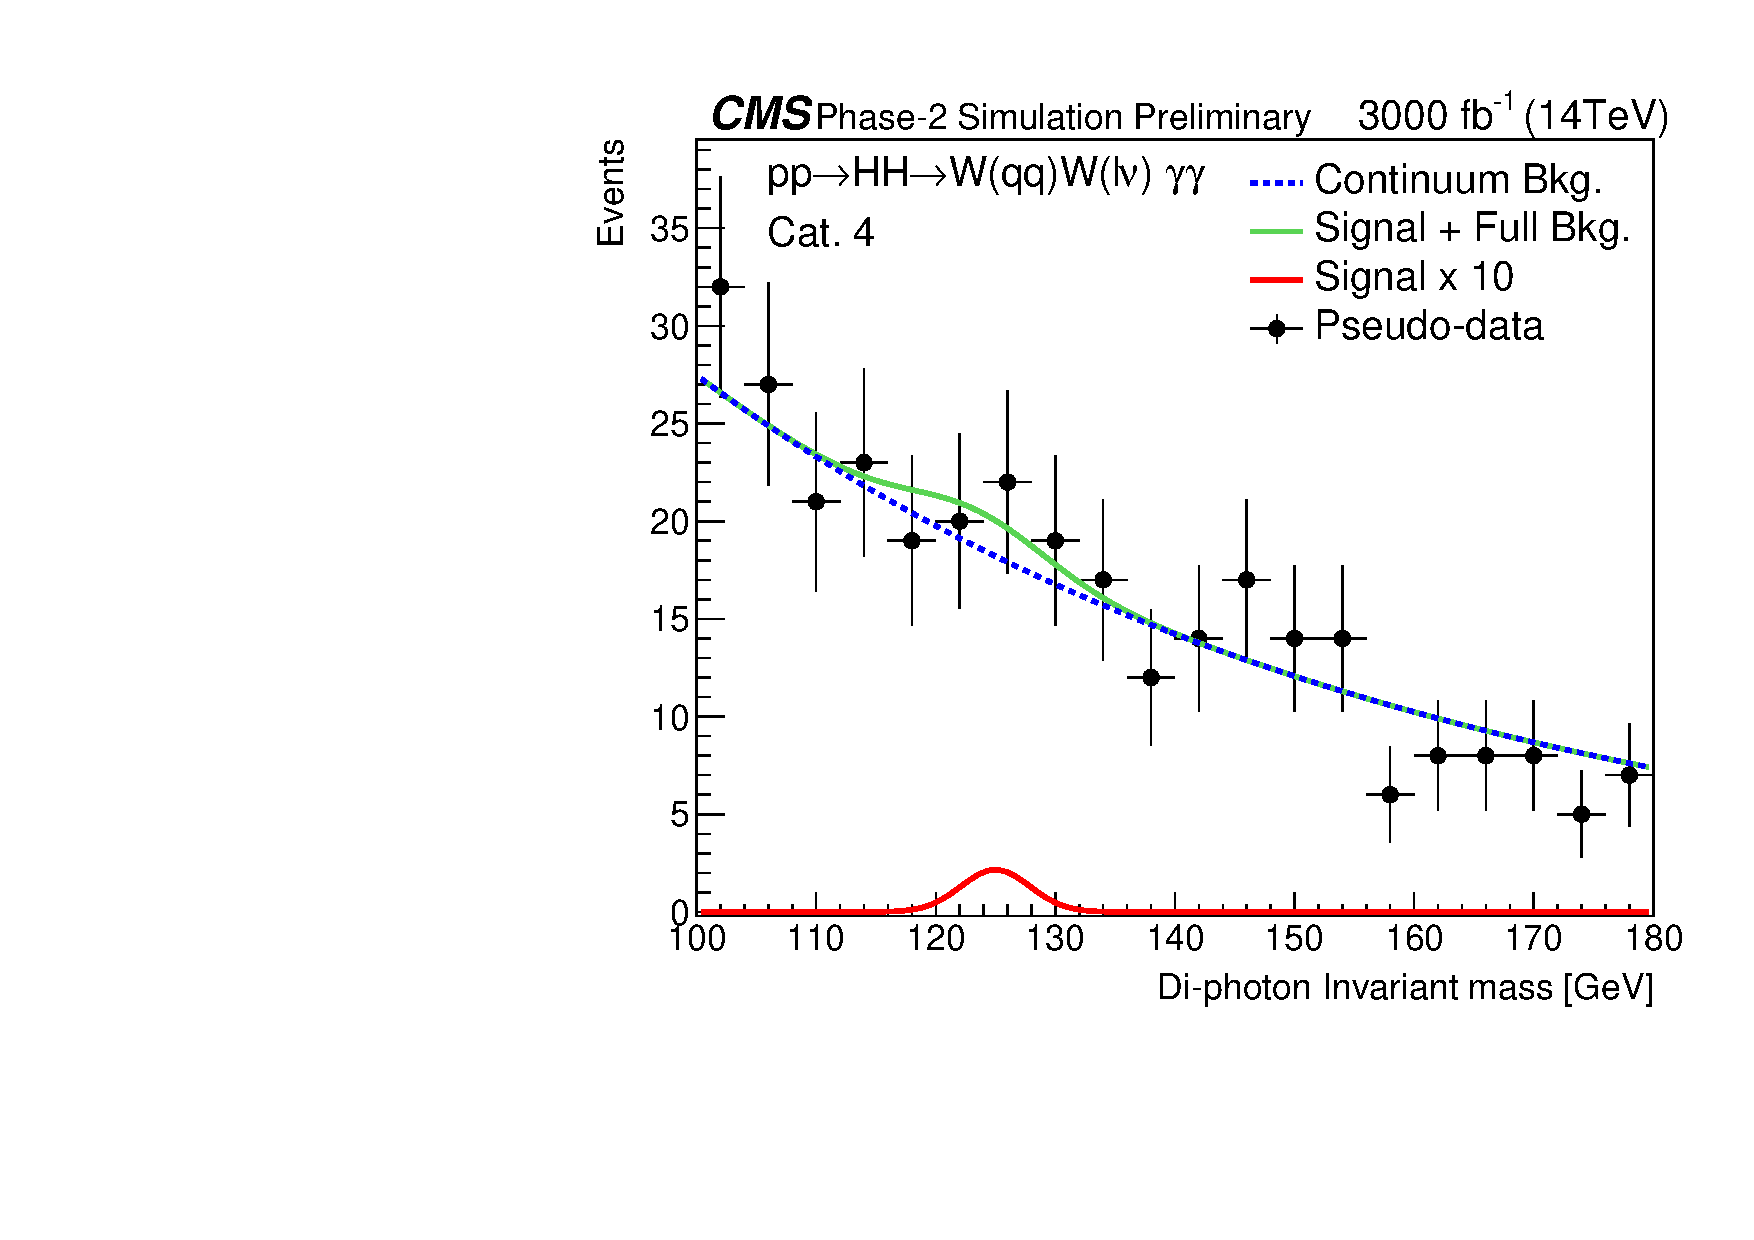
\includegraphics[width=\textwidth]{Inv_mass_gghasOneL_DNN_4_HL_FIT.pdf}
        \vspace{0.1cm}
        %\firstsubcaption{No selection}
    \end{subfigure}
    \hspace{0.2cm}
    \begin{subfigure}[b]{0.475\textwidth}  
        \centering 
        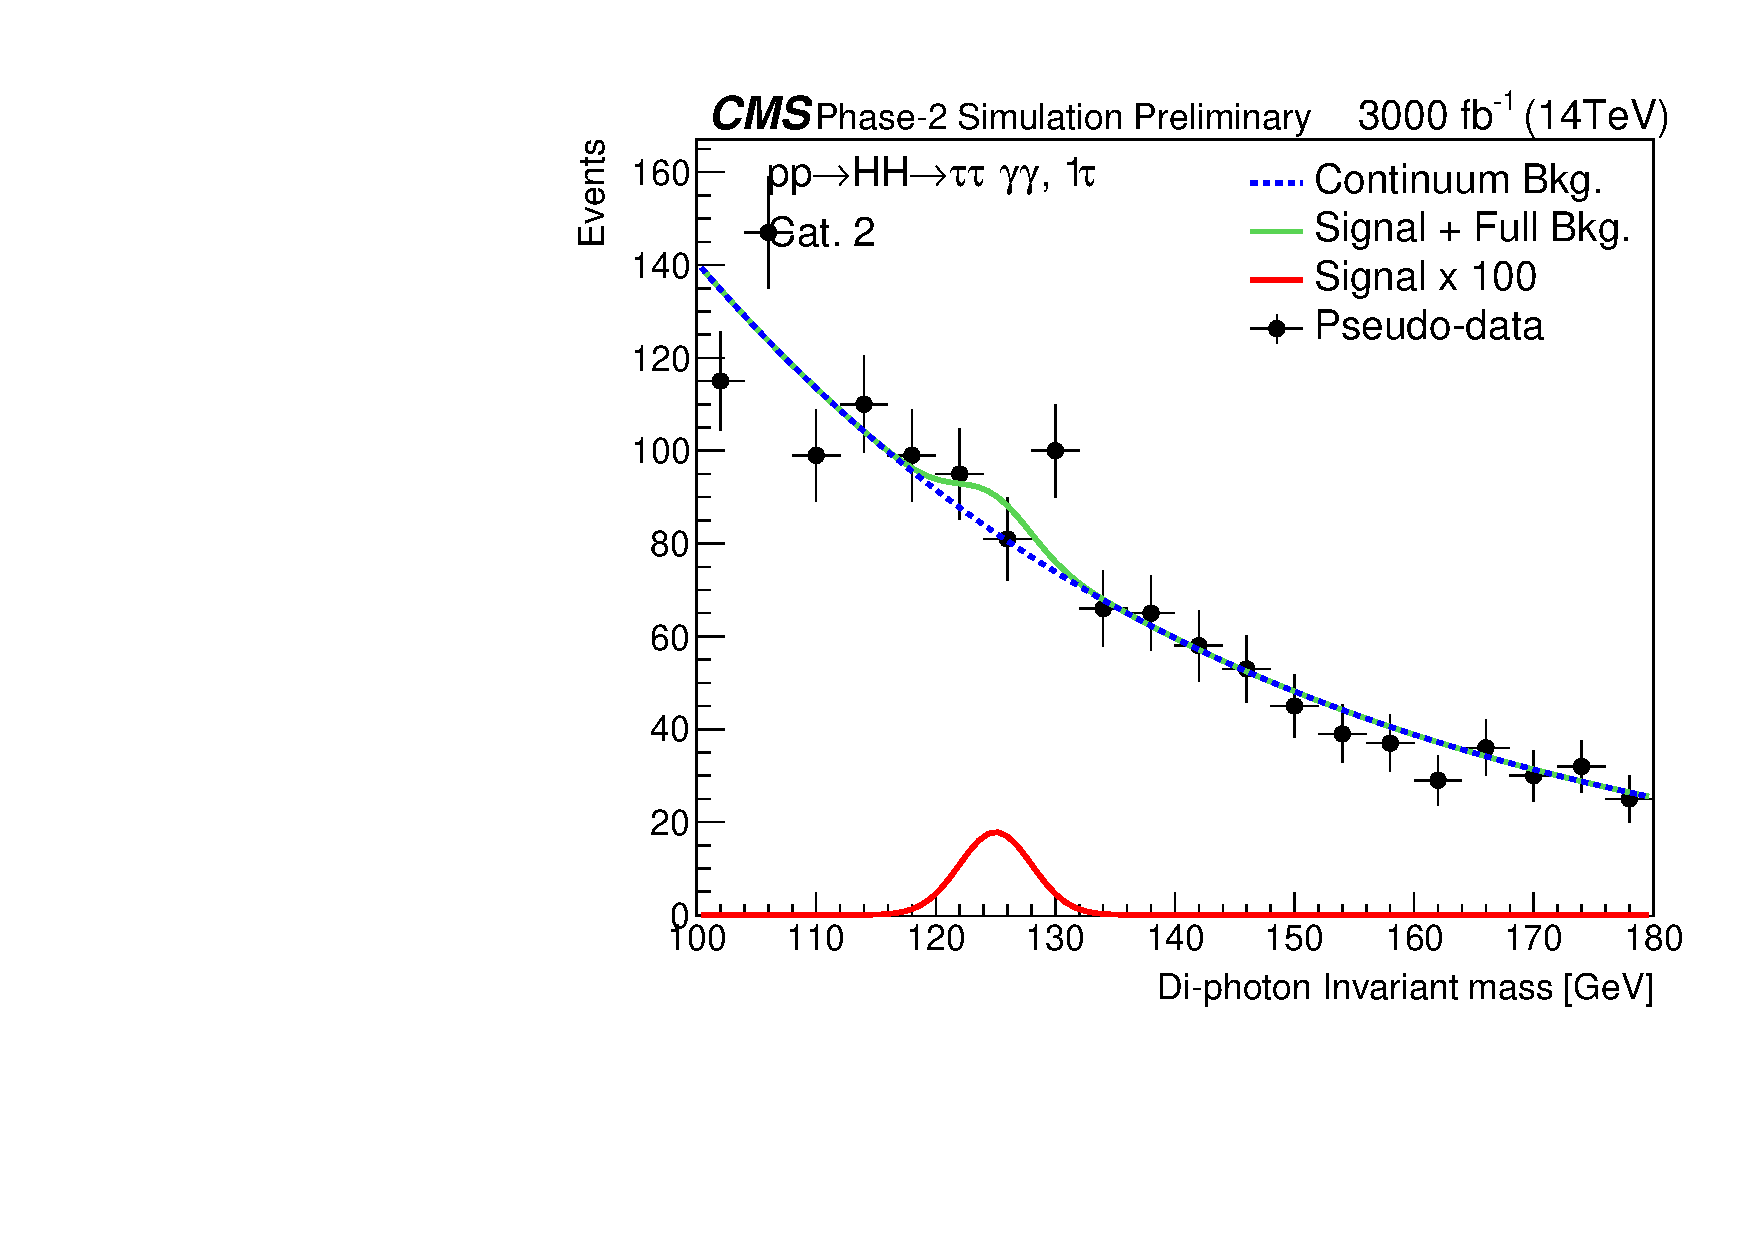
\includegraphics[width=\textwidth]{Mgg_c3_DNN_2_HL_FIT.pdf}
        \vspace{0.1cm}
        %\firstsubcaption{Preselection}
    \end{subfigure}
    \caption[]
    {\small \mgg fit distributions in the semi-leptonic final state's DNN category 4 (left) and in the single $\tau$ final state's DNN category 2 (right).}
    \label{fits}
\end{figure*}